\chapter{Hàm phân phối thực nghiệm và nguyên lý thế}\label{ch:edf}
\section{Từ dữ liệu đến một phân phối}
Với mẫu i.i.d. từ một CDF bất kỳ $F$, định nghĩa
\[
\boxed{\Fhat(x)=\frac1n\sum_{i=1}^n\1_{\{X_i\leq x\}}.}
\]
Mỗi điểm dữ liệu được gán khối lượng $1/n$; nếu giá trị xuất hiện $k$ lần,
bước nhảy tại đó cao $k/n$. Hàm không giảm, liên tục phải, bằng 0 dưới
giá trị nhỏ nhất và bằng 1 từ giá trị lớn nhất trở đi.

\begin{example}
Với $X=(1,2,4,5)$,
\[
\Fhat(x)=\begin{cases}
0,&x<1,\\1/4,&1\leq x<2,\\1/2,&2\leq x<4,\\
3/4,&4\leq x<5,\\1,&x\geq5.
\end{cases}
\]
Vì định nghĩa dùng $\leq$, $\Fhat(2)=1/2$, còn
$\Fhat(2-)=1/4$. Xác suất thực nghiệm của $(2,4]$ bằng $1/4$;
của $[2,4]$ bằng $1/2$ vì khoảng thứ hai có thêm điểm 2.
\end{example}
\intuition{EDF trả lời câu hỏi ``tỷ lệ dữ liệu không vượt quá ngưỡng này
là bao nhiêu?''. Nó không cần chọn ô hay bandwidth và không cần giả thiết
phân phối có mật độ.}
\source{\cite{slide1}, slide 10--17; \cite{wasserman}, Chương 2}

\section{Kỳ vọng, phương sai và hiệp phương sai}
\begin{proposition}
Với mỗi $x,y$ cố định,
\begin{align*}
\E\Fhat(x)&=F(x),\\
\Var\Fhat(x)&=\frac{F(x)[1-F(x)]}{n},\\
\Cov(\Fhat(x),\Fhat(y))
&=\frac{F(\min(x,y))-F(x)F(y)}n.
\end{align*}
\end{proposition}
\begin{proof}
Đặt $I_i(x)=\1_{\{X_i\leq x\}}$. Với $x$ cố định,
$I_i(x)\sim\operatorname{Bernoulli}(F(x))$. Do đó
\[
\E\Fhat(x)=\frac1n\sum_i\E I_i(x)=\frac{nF(x)}n=F(x).
\]
Các $I_i(x)$ độc lập theo chỉ số quan sát, nên
\[
\Var\Fhat(x)=\frac1{n^2}\sum_i\Var I_i(x)
=\frac{nF(x)[1-F(x)]}{n^2}.
\]
Khi xét hai ngưỡng, phải giữ hiệp phương sai của chỉ báo từ cùng một
quan sát:
\begin{align*}
\Cov(\Fhat(x),\Fhat(y))
&=\frac1{n^2}\sum_{i,k}\Cov(I_i(x),I_k(y))\\
&=\frac1{n^2}\sum_i\Cov(I_i(x),I_i(y))\\
&=\frac1n\{\E[I_1(x)I_1(y)]-F(x)F(y)\}.
\end{align*}
Với $i\ne k$, độc lập của $X_i,X_k$ làm hạng chéo bằng 0.
Tích hai chỉ báo bằng $\1_{\{X_1\leq\min(x,y)\}}$, vì đồng thời thỏa
cả hai bất đẳng thức tương đương thỏa ngưỡng nhỏ hơn. Lấy kỳ vọng cho
kết quả. Đặc biệt, nếu $x<y$ thì
\[
\boxed{\Cov(\Fhat(x),\Fhat(y))=\frac{F(x)[1-F(y)]}{n}.}
\]
\end{proof}
\begin{example}
Nếu $n=100$, $F(x)=0.2$, $F(y)=0.7$, $x<y$, thì phương sai tại $x$
là $0.0016$, độ lệch chuẩn $0.04$, và hiệp phương sai hai điểm là
$0.0006$. Các giá trị của đường EDF không độc lập.
\end{example}
\intuition{Nếu một mẫu có nhiều điểm nhỏ hơn $x$, nó cũng có xu hướng có
nhiều điểm nhỏ hơn $y>x$. Do các sự kiện lồng nhau, hiệp phương sai không âm.}

\section{Nhất quán và CLT tại một điểm}
\begin{proposition}
Với mỗi $x$ cố định, $\Fhat(x)\xrightarrow{a.s.}F(x)$. Nếu
$0<F(x)<1$ thì
\[
\boxed{\sqrt n[\Fhat(x)-F(x)]\Rightarrow
N(0,F(x)[1-F(x)]).}
\]
\end{proposition}
\begin{proof}
LLN áp dụng cho các chỉ báo i.i.d. vì $\E|I_i(x)|\leq1$.
CLT áp dụng vì phương sai $F(x)[1-F(x)]$ hữu hạn và dương.
Nếu $F(x)=0$ hoặc 1, các chỉ báo bằng cùng một hằng số gần chắc chắn,
nên sai số bằng 0, không có phân phối chuẩn không suy biến.
\end{proof}
Một khoảng Wald tại điểm, khi cỡ mẫu và tần suất đủ lớn, là
\[
\left[\Fhat(x)-z_{1-\alpha/2}
\sqrt{\frac{\Fhat(x)[1-\Fhat(x)]}{n}},\quad
\Fhat(x)+z_{1-\alpha/2}
\sqrt{\frac{\Fhat(x)[1-\Fhat(x)]}{n}}\right]\cap[0,1].
\]
Đây là xấp xỉ cho một ngưỡng cố định. Nếu $n$ nhỏ hoặc xác suất gần 0, 1,
khoảng Wald có thể rất kém; bài toán tại điểm chính là khoảng tin cậy
cho xác suất nhị thức, có thể dùng Wilson hoặc khoảng nhị thức chính xác.
\intuition{Sai số EDF tại một ngưỡng thường ở thang $n^{-1/2}$.
Giảm một nửa độ lệch chuẩn thường đòi tăng cỡ mẫu bốn lần.}

\section{Hội tụ đều và băng tin cậy DKW}
\begin{theorem}[Dvoretzky--Kiefer--Wolfowitz]
Với mẫu i.i.d. và mọi $\epsilon>0$,
\[
\boxed{\Pp\left(\sup_{x\in\R}|\Fhat(x)-F(x)|>\epsilon\right)
\leq 2e^{-2n\epsilon^2}.}
\]
Không yêu cầu $F$ liên tục.
\end{theorem}
Đây là bất đẳng thức xác suất được viện dẫn. Chứng minh đầy đủ hằng số
tối ưu 2 vượt quá phần nền; dưới đây chứng minh các hệ quả cần sử dụng.

\begin{theorem}[Glivenko--Cantelli]
$\sup_x|\Fhat(x)-F(x)|\xrightarrow{a.s.}0$.
\end{theorem}
\begin{proof}
Đặt $Z_n=\sup_x|\Fhat(x)-F(x)|$. Với mỗi số nguyên $k\geq1$,
\[
\sum_{n=1}^\infty\Pp(Z_n>1/k)
\leq2\sum_{n=1}^\infty e^{-2n/k^2}<\infty,
\]
vì vế phải là chuỗi hình học có công bội nhỏ hơn 1.
Bổ đề Borel--Cantelli thứ nhất cho biết $Z_n>1/k$ chỉ xảy ra hữu hạn
lần, gần chắc chắn. Giao các sự kiện xác suất 1 này trên $k=1,2,\ldots$
vẫn có xác suất 1. Trên giao đó, với mọi $\epsilon>0$, chọn $k$ sao cho
$1/k<\epsilon$; từ một chỉ số trở đi $Z_n\leq1/k<\epsilon$.
Đó chính là hội tụ gần chắc chắn về 0.
\end{proof}

\step{Dựng băng đồng thời.}
Giải $2e^{-2n\epsilon_n^2}=\alpha$:
\[
\epsilon_n=\sqrt{\frac{\log(2/\alpha)}{2n}},\quad
L_n(x)=\max\{0,\Fhat(x)-\epsilon_n\},\quad
U_n(x)=\min\{1,\Fhat(x)+\epsilon_n\}.
\]
Trên sự kiện $Z_n\leq\epsilon_n$, bất đẳng thức
$\Fhat(x)-\epsilon_n\leq F(x)\leq\Fhat(x)+\epsilon_n$ đúng
\emph{đồng thời cho mọi $x$}. Cắt tại 0 và 1 không làm mất giá trị thật
vì $0\leq F(x)\leq1$. Vì vậy
\[
\boxed{\Pp(\forall x:\ L_n(x)\leq F(x)\leq U_n(x))\geq1-\alpha.}
\]
Mức bao phủ ít nhất $1-\alpha$, không nhất thiết đúng bằng mức đó.
Với $n=100$, $\alpha=0.05$, $\epsilon_n\approx0.13581$.
Nếu muốn nửa độ rộng không vượt $\delta$, cần
$n\geq\lceil\log(2/\alpha)/(2\delta^2)\rceil$;
với $\delta=0.05$, mức 95\%, cần $n\geq738$.

\begin{figure}[htbp]
\centering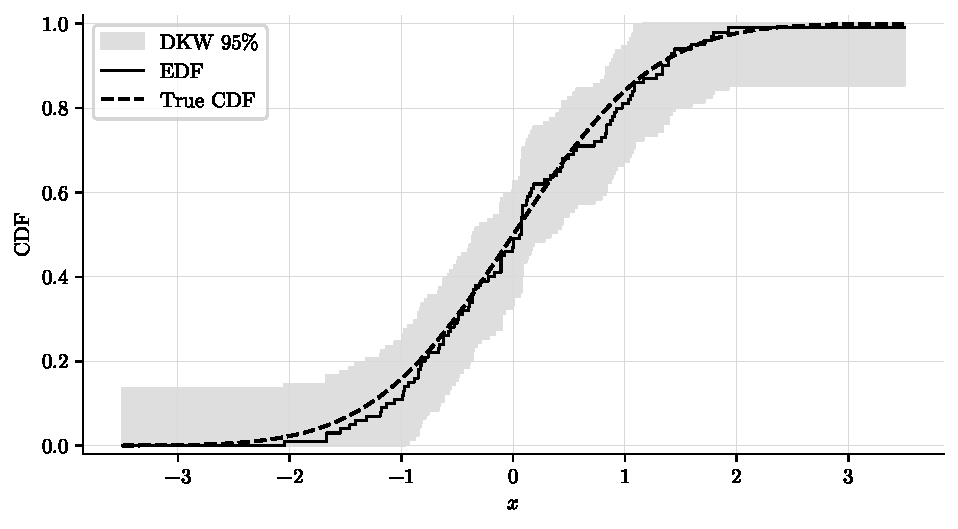
\includegraphics[width=.88\textwidth]{edf_dkw.pdf}
\caption{EDF và băng DKW 95\% trên một mẫu chuẩn mô phỏng, $n=100$.
Đường liền là CDF thật để đối chiếu; băng tính từ dữ liệu. Một hình
đơn lẻ không chứng minh mức bao phủ qua các mẫu lặp lại.}
\end{figure}
\intuition{Khoảng tại điểm là bảo đảm cho một ngưỡng; băng DKW là bảo đảm
cho toàn bộ đường. Cùng mức tin cậy, yêu cầu đồng thời thường cần băng rộng hơn.}
\pitfall{Lấy 100 khoảng Wald mức 95\% không tạo ra một băng đồng thời 95\%.
EDF có bước nhảy không làm DKW mất hiệu lực.}
\source{\cite{slide1}, slide 16--20; \cite{wasserman}, Chương 2}

\section{Functional và nguyên lý thế}
Một \emph{functional} là ánh xạ từ phân phối thành một số hoặc vectơ:
$T:F\mapsto T(F)$. Nguyên lý thế định nghĩa
\[
\boxed{\widehat\theta=T(\Fhat).}
\]
Nếu $T$ liên tục tại $F$ theo chuẩn sup của CDF thì Glivenko--Cantelli
và tính liên tục cho $T(\Fhat)\xrightarrow{a.s.}T(F)$.
Tính liên tục là giả thiết, không phải tính chất của mọi functional.
Chẳng hạn trung bình trên miền không bị chặn không liên tục theo chuẩn sup:
$F_m=(1-1/m)\delta_0+(1/m)\delta_{m^2}$ cách $\delta_0$ không quá
$1/m$ về CDF, nhưng trung bình của $F_m$ bằng $m$. Trung bình mẫu vẫn
nhất quán khi moment tuyệt đối bậc nhất hữu hạn, nhờ LLN.

\subsection{Functional tuyến tính}
Với $T(F)=\int a(x)\,dF(x)$ và $\E|a(X)|<\infty$,
\[
T(\Fhat)=\int a(x)\frac1n\sum_i\delta_{X_i}(dx)
=\frac1n\sum_ia(X_i).
\]
Tích phân theo khối lượng điểm $\delta_{X_i}$ bằng giá trị hàm tại $X_i$.
Từ LLN, ước lượng nhất quán; từ tuyến tính của kỳ vọng, không chệch.
Nếu $\Var(a(X))<\infty$,
\[
\Var(T(\Fhat))=\frac{\Var(a(X))}{n},\qquad
\sqrt n[T(\Fhat)-T(F)]\Rightarrow N(0,\Var(a(X))).
\]
Trung bình, moment thô và xác suất một tập cố định là những ví dụ.

\subsection{Trung bình, phương sai và độ lệch}
Đặt $\mu=\int x\,dF$, $\sigma^2=\int(x-\mu)^2\,dF$.
\[
\widehat\mu=\overline X,\qquad
\widehat\sigma^2_{\rm plug}=\frac1n\sum_i(X_i-\overline X)^2
=\overline{X^2}-\overline X^2.
\]
Functional phương sai phi tuyến vì $\mu$ cũng phụ thuộc $F$.
Từ $\E\overline{X^2}=\sigma^2+\mu^2$ và
$\E\overline X^2=\sigma^2/n+\mu^2$, suy ra
\[
\E\widehat\sigma^2_{\rm plug}=\frac{n-1}{n}\sigma^2.
\]
Ước lượng không chệch là $s^2=(n-1)^{-1}\sum_i(X_i-\overline X)^2$,
không phải đúng estimator plug-in của functional phương sai.
Cả hai nhất quán nếu $\E X^2<\infty$.

Skewness của phân phối có $\sigma>0$ và moment tuyệt đối bậc ba hữu hạn:
\[
\gamma_1(F)=\frac{\E(X-\mu)^3}{\sigma^3},\qquad
\widehat\gamma_1=\frac{n^{-1}\sum_i(X_i-\overline X)^3}
{[n^{-1}\sum_i(X_i-\overline X)^2]^{3/2}}.
\]
Nếu phương sai mẫu bằng 0, tỷ số không xác định. Các phiên bản hiệu chỉnh
skewness trong phần mềm có thể khác công thức plug-in này.
\begin{example}
Với $(1,2,4,5)$, $\overline X=3$, tổng bình phương độ lệch là 10.
Phương sai plug-in là $2.5$, $s^2=10/3$. Tổng lập phương độ lệch là
$-8-1+1+8=0$, nên skewness plug-in bằng 0.
\end{example}

\subsection{Tương quan và quantile}
Với mẫu cặp $(X_i,Y_i)$, dùng \emph{phân phối thực nghiệm đồng thời}.
Khi hai phương sai dương,
\[
\widehat\rho=
\frac{\sum_i(X_i-\overline X)(Y_i-\overline Y)}
{\sqrt{\sum_i(X_i-\overline X)^2\sum_i(Y_i-\overline Y)^2}}.
\]
Các hệ số $1/n$ triệt tiêu giữa tử và mẫu. Không thể khôi phục tương quan
chỉ từ hai CDF biên: cần cấu trúc phụ thuộc của các cặp.

Với $0<p<1$, quantile là nghịch đảo suy rộng:
\[
q_p=\inf\{x:F(x)\geq p\},\qquad
\widehat q_p=\inf\{x:\Fhat(x)\geq p\}=X_{(\lceil np\rceil)}.
\]
Đây là quy ước quantile dùng xuyên suốt tài liệu. Với mẫu bốn điểm trên,
$\widehat q_{0.5}=2$, khác trung vị nội suy $3$ thường dùng trong mô tả.
Nếu $F$ có quantile duy nhất và liên tục, tăng thực sự quanh $q_p$,
ước lượng quantile nhất quán. Nếu thêm $f(q_p)>0$ và $f$ liên tục gần đó,
biểu diễn tuyến tính tiệm cận là
\[
\widehat q_p-q_p=
-\frac{\Fhat(q_p)-p}{f(q_p)}+o_P(n^{-1/2}),
\quad
\sqrt n(\widehat q_p-q_p)\Rightarrow
N\left(0,\frac{p(1-p)}{f(q_p)^2}\right).
\]
Đây là kết quả được viện dẫn về quantile; trực giác đến từ
$F(q_p+t)\approx p+f(q_p)t$. Sai số theo chiều đứng của EDF được chia
cho độ dốc để đổi sang sai số theo chiều ngang. Mật độ nhỏ quanh quantile
làm sai số vị trí lớn.
\intuition{Plug-in biến một phân phối thực nghiệm thành thống kê quen thuộc.
Tính đúng đắn của suy luận phụ thuộc moment, tính liên tục và mẫu số của
functional, không chỉ phụ thuộc EDF hội tụ.}
\source{\cite{slide1}, slide 30--35; \cite{wasserman}, Chương 2}

\section{Kiểm định sự phù hợp}
Xét $H_0:F=F_0$ với $F_0$ \emph{liên tục, được chỉ định đầy đủ}.
Khi đó $U_i=F_0(X_i)$ i.i.d. đều trên $[0,1]$ dưới $H_0$.
Điều này giải thích tính không phụ thuộc phân phối của các thống kê sau.

\subsection{Kolmogorov--Smirnov}
\[
D_n=\sup_x|\Fhat(x)-F_0(x)|.
\]
Với $X_{(1)}\leq\cdots\leq X_{(n)}$, cần kiểm tra hai phía của mỗi
bước nhảy. Trong các khoảng không có dữ liệu, EDF hằng còn $F_0$ không
giảm; độ lệch lớn nhất đạt ở giới hạn hai đầu khoảng. Vì vậy
\begin{align*}
D_n^+&=\max_i\left\{\frac in-F_0(X_{(i)})\right\},\\
D_n^-&=\max_i\left\{F_0(X_{(i)})-\frac{i-1}n\right\},\qquad
\boxed{D_n=\max(D_n^+,D_n^-).}
\end{align*}
DKW cho kiểm định bảo thủ hữu hạn mẫu: bác bỏ khi
$D_n>\sqrt{\log(2/\alpha)/(2n)}$.
Với phân phối liên tục, giới hạn của $\sqrt nD_n$ là
$\sup_{0\leq t\leq1}|B(t)|$, với $B$ là cầu Brown.
\[
\Pp\big(\sup_t|B(t)|>z\big)
=2\sum_{k=1}^{\infty}(-1)^{k-1}e^{-2k^2z^2},\quad z>0.
\]
Đây là định lý giới hạn được viện dẫn. Mốc tiệm cận 95\% thường dùng
là $1.358/\sqrt n$; cần bảng hoặc thuật toán chính xác khi mẫu nhỏ.

\subsection{Cramér--von Mises}
CvM đo sai khác bình phương, tích phân theo $F_0$:
\[
W_n^2=n\int[\Fhat(x)-F_0(x)]^2\,dF_0(x)
=\frac1{12n}+\sum_{i=1}^n
\left[F_0(X_{(i)})-\frac{2i-1}{2n}\right]^2.
\]
Để thấy nguồn gốc công thức, đặt $u_i=F_0(X_{(i)})$, $u_0=0$,
$u_{n+1}=1$. CDF thực nghiệm trên $(u_i,u_{i+1})$ bằng $i/n$:
\[
W_n^2=n\sum_{i=0}^n\int_{u_i}^{u_{i+1}}(i/n-t)^2\,dt.
\]
Lấy nguyên hàm $t^3/3-(i/n)t^2+(i/n)^2t$ và thu gọn các đầu mút,
ta được $n/3+\sum_i[u_i^2-(2i-1)u_i/n]$.
Hoàn thành bình phương từng hạng và dùng
$\sum_i(2i-1)^2=n(4n^2-1)/3$ cho công thức trên.

\subsection{Anderson--Darling}
AD tăng trọng số ở hai đuôi:
\[
A_n^2=n\int\frac{[\Fhat(x)-F_0(x)]^2}
{F_0(x)[1-F_0(x)]}\,dF_0(x).
\]
Khi $0<u_i<1$, công thức tính là
\[
\boxed{A_n^2=-n-\frac1n\sum_{i=1}^n(2i-1)
\{\log u_i+\log(1-u_{n+1-i})\}.}
\]
Có thể kiểm tra bằng chia khoảng như CvM và phân tích
\[
\frac{(c-t)^2}{t(1-t)}
=\frac{c^2}{t}+\frac{(1-c)^2}{1-t}-1.
\]
Nguyên hàm là $c^2\log t-(1-c)^2\log(1-t)-t$.
Thế $c=i/n$ trên từng khoảng; hiệu hệ số ở một đầu mút cho các trọng số
$(2i-1)/n$. Ở khoảng sát 0 hoặc 1, hệ số đi với log phân kỳ bằng 0;
lấy giới hạn một phía để thu gọn. Nếu dữ liệu có $u_i=0$ hoặc 1,
AD có thể vô hạn: không tùy ý thay log 0 bằng 0.

\begin{center}
\begin{tabular}{lll}
\toprule Kiểm định & Đo sai khác & Nhấn mạnh\\\midrule
KS & Sai khác lớn nhất & Vị trí lệch nhiều nhất\\
CvM & Bình phương tích phân & Sai khác trên toàn miền\\
AD & Bình phương có trọng số & Hai đuôi\\\bottomrule
\end{tabular}
\end{center}
\intuition{KS nhìn điểm tệ nhất; CvM cộng sai khác; AD phóng đại sai khác
ở những vùng CDF gần 0 hoặc 1. Không có thống kê tốt nhất cho mọi đối thuyết.}
\pitfall{Nếu dùng mẫu để ước lượng $\mu,\sigma$ rồi kiểm định với
$N(\widehat\mu,\widehat\sigma^2)$, bảng KS chuẩn không còn đúng. Cần
hiệu chỉnh tương ứng hoặc bootstrap tham số có bước fit lại trong mỗi lần
lặp. Với $F_0$ rời rạc, phân phối null cũng khác. Không bác bỏ $H_0$
không có nghĩa chứng minh $H_0$ đúng.}
\source{\cite{slide1}, slide 36--46}

\section{Tự kiểm tra trước khi sang Chương 2}
Bạn cần tự làm được: viết EDF có dữ liệu trùng; phân biệt $F_n(x)$ và
$F_n(x-)$; chứng minh covariance bằng tích chỉ báo; suy ra băng DKW;
giải thích vì sao phương sai plug-in có mẫu số $n$; tính KS bằng cả
$D_n^+$ và $D_n^-$. Chương 6 có ba bài KS và một bài EDF/DKW để luyện.
